% !TeX program = lualatex
% O template exige LuaLaTeX (fontspec com as fontes de fontes/). Editores que
% respeitam este magic comment escolhem o motor sozinhos; nos que não respeitam,
% selecione LuaLaTeX na configuração de compilador do projeto.

\documentclass[a4paper,11pt,twoside]{article}

\usepackage[brazilian]{babel}
\usepackage[code,smartrefs,floatbarriers]{poliusp}

% Dados da capa e do cabeçalho — edite capa.tex
% ==============================================================
%  DADOS DO RELATÓRIO
%  Edite apenas este arquivo para configurar a capa e o cabeçalho.
% ==============================================================

\titulo[Zovic -- Banco de Dados]{Zovic:\\Banco de Dados}

\subtitulo{Modelo conceitual, modelo relacional e evolução do esquema}

% Um autor por linha, separados por \\. Complete os nomes e os números USP.
\Autores{
    Caio -- NUSP XXXXXXX\\
    Carlos -- NUSP XXXXXXX\\
    Felipe Labrego Argolo -- NUSP XXXXXXX\\
    Gabriel -- NUSP XXXXXXX\\
    Victor Bertelli -- NUSP XXXXXXX
}

\departamento{Departamento de Engenharia de Computação e Sistemas Digitais}

\disciplina{Engenharia de Software}

\data{novembro de 2026}


% Colunas de tabela com largura proporcional e alinhadas à esquerda,
% no mesmo estilo das tabelas do template.
\newcolumntype{L}[1]{>{\raggedright\arraybackslash\hsize=#1\hsize}X}
% Nome de tabela, coluna ou arquivo; pode quebrar a linha depois de _, . e /.
\DeclareRobustCommand{\campo}[1]{\begingroup\ttfamily\let\poliSublinhado\_%
  \renewcommand{\_}{\poliSublinhado\allowbreak}\poliBarras#1/\poliFim\endgroup}
\def\poliBarras#1/#2\poliFim{\poliPontos#1.\poliFimPonto\ifx\relax#2\relax\else/\allowbreak\poliBarras#2\poliFim\fi}
\def\poliPontos#1.#2\poliFimPonto{#1\ifx\relax#2\relax\else.\allowbreak\poliPontos#2\poliFimPonto\fi}
% Folga extra entre palavras antes de deixar uma linha passar da margem.
\setlength{\emergencystretch}{3em}

\begin{document}

\tableofcontents
\clearpage

\section{Introdução}

O Zovic é uma plataforma de streaming de música desenvolvida na disciplina de
Engenharia de Software. Visitantes navegam pelo catálogo, assinantes ouvem
músicas, montam playlists, comentam e avaliam faixas, e um gestor pode dividir
um plano familiar com até quatro pessoas. Um administrador mantém o catálogo e
acompanha as estatísticas de uso.

Todos esses dados ficam num único banco PostgreSQL. Este relatório descreve
como ele foi modelado e como é mantido:

\begin{itemize}
  \item o \textbf{modelo conceitual} (\cref{sec:conceitual}), que mostra as
    entidades do domínio e como elas se relacionam, sem detalhes de
    implementação;
  \item o \textbf{modelo relacional} (\cref{sec:relacional}), que mapeia o
    conceitual em tabelas, chaves primárias e chaves estrangeiras;
  \item as \textbf{restrições de integridade} (\cref{sec:integridade}) que o
    próprio banco garante;
  \item a \textbf{evolução do esquema} por migrations (\cref{sec:evolucao}) e
    o \textbf{acesso aos dados} pela API (\cref{sec:acesso});
  \item as \textbf{limitações conhecidas} e o que ainda está planejado
    (\cref{sec:limitacoes}).
\end{itemize}

A fonte da verdade do esquema são as migrations em \campo{db/migrations/}, no
repositório do projeto. Este relatório acompanha a última delas,
\campo{V261117\_170000\_\_Adiciona\_imagem\_da\_playlist\_e\_do\_artista.sql}.

\section{Tecnologias e Organização}
\label{sec:tecnologias}

\begin{table}[htbp]
  \centering
  \caption{Ferramentas usadas no banco de dados}
  \label{tab:ferramentas}
  \begin{tabularx}{\textwidth}{@{}L{0.6}L{1.4}@{}}
    \toprule
    \poliCabTabela{Ferramenta} & \poliCabTabela{Papel} \\
    \midrule
    PostgreSQL 16 & Sistema gerenciador do banco, local (Docker) e em produção \\
    Flyway & Cria e altera o esquema com migrations em SQL, numeradas pela data e hora \\
    \campo{pg} (node-postgres) & Driver usado pela API para executar o SQL dos repositórios \\
    Prisma & Client tipado, gerado a partir do banco, usado no seed e nos testes \\
    Better Auth & Biblioteca de autenticação; usa as tabelas \campo{user}, \campo{session}, \campo{account} e \campo{verification} \\
    D2 & Desenha o diagrama do banco a partir do próprio Postgres, a cada push \\
    \bottomrule
  \end{tabularx}
\end{table}

A divisão de responsabilidades é estrita: \textbf{só o Flyway altera o
esquema}. O Prisma apenas espelha o banco (\campo{prisma db pull}), e o Better
Auth nunca cria tabelas sozinho. Quando a biblioteca precisa de uma coluna
nova, a equipe escreve uma migration com as convenções do projeto. Assim, há
um único histórico de mudanças, e qualquer máquina chega ao mesmo esquema
aplicando as migrations em ordem.

A API segue a arquitetura de portas e adaptadores. As regras de negócio ficam
em \campo{api/domain}, que declara \emph{portas} (interfaces como
\campo{PlaylistRepository}) sem conhecer o banco. As implementações em SQL
ficam em \campo{api/adapters/db}, uma por porta, como
\campo{PostgresPlaylistRepository}. Isso permite testar os casos de uso com
repositórios em memória e testar os adaptadores contra um Postgres real.

\section{Modelo Conceitual}
\label{sec:conceitual}

O modelo conceitual descreve \emph{o que} o sistema guarda, sem decidir
\emph{como}. Ele usa a notação de Chen, no estilo do brModelo: as entidades
ficam em retângulos, os relacionamentos em losangos e os atributos em
círculos, com o identificador em preto. A cardinalidade (mín, máx)
junto de uma entidade diz quantas instâncias dela se ligam a
\emph{uma} instância da outra ponta. Em \emph{assina}, por exemplo, o
(1,n) junto de Usuário diz que todo plano tem ao menos uma pessoa, e o
(0,n) junto de Plano diz que uma conta pode existir sem plano.

\begin{figure}[htbp]
  \centering
  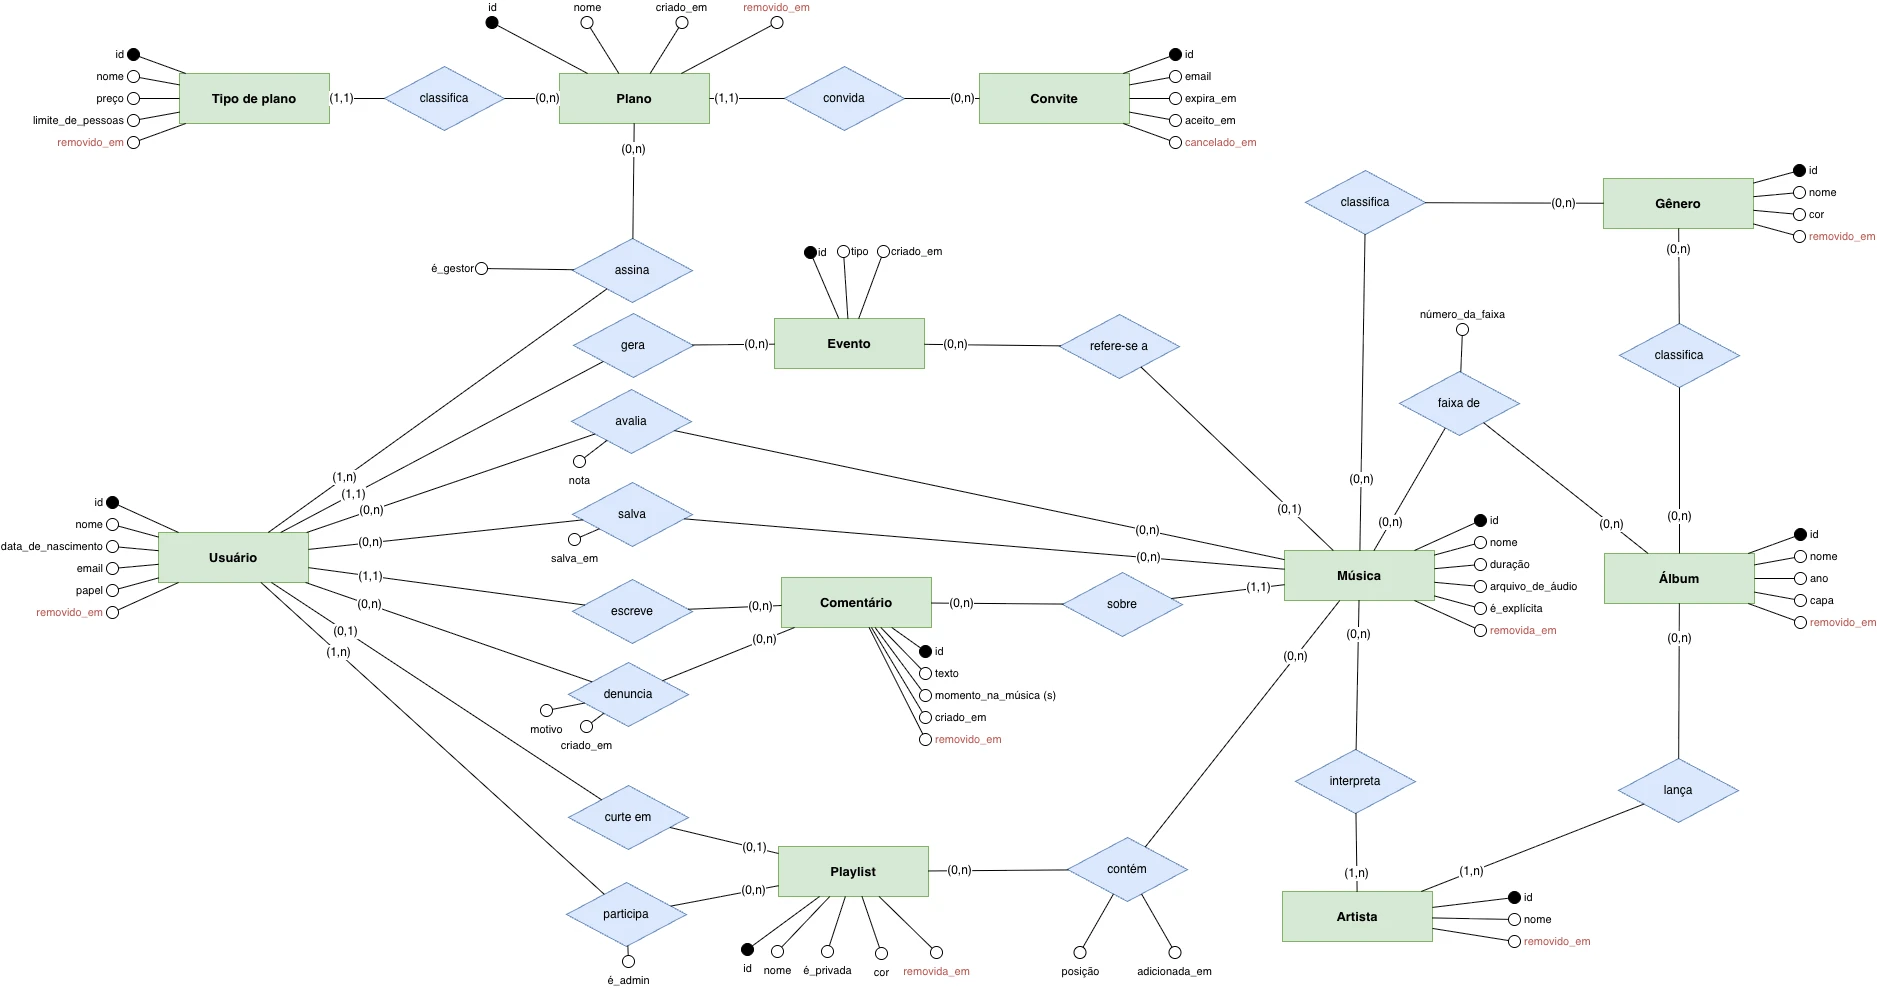
\includegraphics[width=\textwidth]{figuras/der-conceitual.png}
  \caption{Diagrama Entidade-Relacionamento conceitual do Zovic}
  \label{fig:der}
\end{figure}

Como o diagrama é conceitual, ele não mostra chaves estrangeiras nem tabelas
associativas. Um relacionamento é desenhado uma única vez, pela linha que liga
as entidades. Quando o vínculo tem dados próprios, eles aparecem como
atributos do losango: a \emph{nota} pertence a \emph{avalia}, e não ao usuário
nem à música; a \emph{posição} de uma faixa pertence a \emph{contém}, porque a
mesma música ocupa posições diferentes em playlists diferentes.

\subsection{Entidades}

\begin{table}[htbp]
  \centering
  \caption{Entidades do modelo conceitual}
  \label{tab:entidades}
  \begin{tabularx}{\textwidth}{@{}L{0.55}L{1.45}@{}}
    \toprule
    \poliCabTabela{Entidade} & \poliCabTabela{O que representa} \\
    \midrule
    Usuário & Uma conta. O papel (\emph{admin} ou \emph{assinante}) define o que ela pode fazer; o visitante não tem conta e não aparece no banco. A data de nascimento decide se a conta vê conteúdo explícito. \\
    Tipo de plano & Uma oferta comercial, com preço e limite de pessoas: Individual (1) e Família (4). \\
    Plano & Uma assinatura de um tipo de plano. \\
    Convite & Um convite do gestor para alguém entrar no plano familiar, com validade. \\
    Música & Uma faixa do catálogo, com duração, arquivo de áudio e a marca de conteúdo explícito. \\
    Álbum & Um lançamento, com ano e capa. \\
    Artista & Quem interpreta músicas e lança álbuns, com foto opcional. \\
    Gênero & Uma classificação de músicas e álbuns, com uma cor para a interface. \\
    Playlist & Uma lista ordenada de músicas, pública ou privada, com capa opcional. \\
    Comentário & Um texto sobre uma música, que pode apontar um momento dela (em segundos). \\
    Evento & Um registro de uso: cadastro, login, logout, reprodução, pulo ou música ouvida. \\
    \bottomrule
  \end{tabularx}
\end{table}

\FloatBarrier
\subsection{Relacionamentos}

\begin{table}[htbp]
  \centering
  \caption{Relacionamentos, cardinalidades e atributos}
  \label{tab:relacionamentos}
  \small
  \begin{tabularx}{\textwidth}{@{}L{0.85}L{1.2}L{0.45}L{1.5}@{}}
    \toprule
    \poliCabTabela{Relacionamento} & \poliCabTabela{Entidades} & \poliCabTabela{Tipo} & \poliCabTabela{Atributos e regras} \\
    \midrule
    classifica & Tipo de plano -- Plano & 1:N & Todo plano tem exatamente um tipo \\
    assina & Usuário -- Plano & N:M & \emph{é\_gestor}; todo plano tem ao menos uma pessoa \\
    convida & Plano -- Convite & 1:N & Todo convite é de um plano \\
    gera & Usuário -- Evento & 1:N & Todo evento é de uma conta \\
    refere-se a & Evento -- Música & N:1 & Opcional: só eventos de reprodução têm música \\
    avalia & Usuário -- Música & N:M & \emph{nota}, de 1 a 5 \\
    salva & Usuário -- Música & N:M & \emph{salva\_em} \\
    escreve & Usuário -- Comentário & 1:N & Todo comentário tem um autor \\
    sobre & Comentário -- Música & N:1 & Todo comentário é de uma música \\
    denuncia & Usuário -- Comentário & N:M & \emph{motivo}, \emph{criado\_em}; uma denúncia por pessoa e comentário \\
    participa & Usuário -- Playlist & N:M & \emph{é\_admin}; toda playlist tem ao menos um membro \\
    curte em & Usuário -- Playlist & 1:1 & A playlist ``Músicas Curtidas'' de cada conta \\
    contém & Playlist -- Música & N:M & \emph{posição}, \emph{adicionada\_em} \\
    faixa de & Música -- Álbum & N:M & \emph{número\_da\_faixa} \\
    interpreta & Artista -- Música & N:M & Toda música tem ao menos um artista \\
    lança & Artista -- Álbum & N:M & Todo álbum tem ao menos um artista \\
    classifica & Gênero -- Música & N:M & -- \\
    classifica & Gênero -- Álbum & N:M & -- \\
    \bottomrule
  \end{tabularx}
\end{table}

\FloatBarrier
\subsection{Decisões de modelagem}

\paragraph{Remoção lógica.} Músicas, álbuns, artistas, gêneros, playlists,
planos, usuários, comentários e avaliações nunca são apagados de verdade.
Removê-los preenche o atributo \emph{removido\_em}, destacado em vermelho na
\cref{fig:der}. Isso preserva o histórico: uma música tirada do catálogo
continua contando nas estatísticas de reprodução, e o email de uma conta
removida continua reservado.

\paragraph{Dados derivados ficam de fora.} O modelo não guarda o que pode ser
calculado a partir de outros dados. A média das notas de uma música sai de
\emph{avalia}, e o número de reproduções sai dos eventos. Guardar esses valores
numa coluna criaria redundância: os dois números poderiam divergir. O mesmo
vale para os totais do sistema (usuários, músicas e playlists), que um
\campo{COUNT} já calcula.

\paragraph{Autenticação é infraestrutura.} As sessões, as credenciais e os
tokens de verificação existem porque o Better Auth precisa deles, e não por
uma regra do negócio. Eles aparecem no modelo relacional, mas não no
conceitual.

\section{Modelo Relacional}
\label{sec:relacional}

O modelo relacional é o modelo lógico: diz como o conceitual vira tabelas no
PostgreSQL. O mapeamento segue três regras:

\begin{enumerate}
  \item \textbf{Cada entidade vira uma tabela}, com uma chave primária
    \campo{id} inteira gerada pelo banco
    (\campo{GENERATED BY DEFAULT AS IDENTITY}).
  \item \textbf{Um relacionamento 1:N vira uma chave estrangeira} no lado N.
    \emph{escreve} vira a coluna \campo{comments.user\_id}, e \emph{convida}
    vira \campo{plan\_invitation.plan\_id}. O relacionamento 1:1 \emph{curte
    em} vira \campo{playlists.liked\_by\_user\_id}, com \campo{UNIQUE} para
    que cada conta tenha uma única playlist de curtidas.
  \item \textbf{Um relacionamento N:M vira uma tabela associativa}, cuja chave
    primária é o par de chaves estrangeiras. Os atributos do relacionamento
    viram colunas dela: \emph{contém} vira \campo{music\_playlist}, com
    \campo{position} e \campo{added\_at}.
\end{enumerate}

\emph{avalia} e \emph{denuncia} são exceções à regra 3: viraram as tabelas
\campo{rating} e \campo{comment\_reports}, com um \campo{id} próprio no lugar
da chave composta. Em \campo{rating}, isso é necessário, porque uma avaliação
removida continua guardada (remoção lógica) e a mesma pessoa pode avaliar a
música de novo; a regra ``uma avaliação ativa por pessoa e música'' fica num
índice único parcial. Em \campo{comment\_reports}, o par
(\campo{comment\_id}, \campo{user\_id}) continua único por uma constraint
\campo{UNIQUE} (\cref{sec:integridade}).

\begin{figure}[htbp]
  \centering
  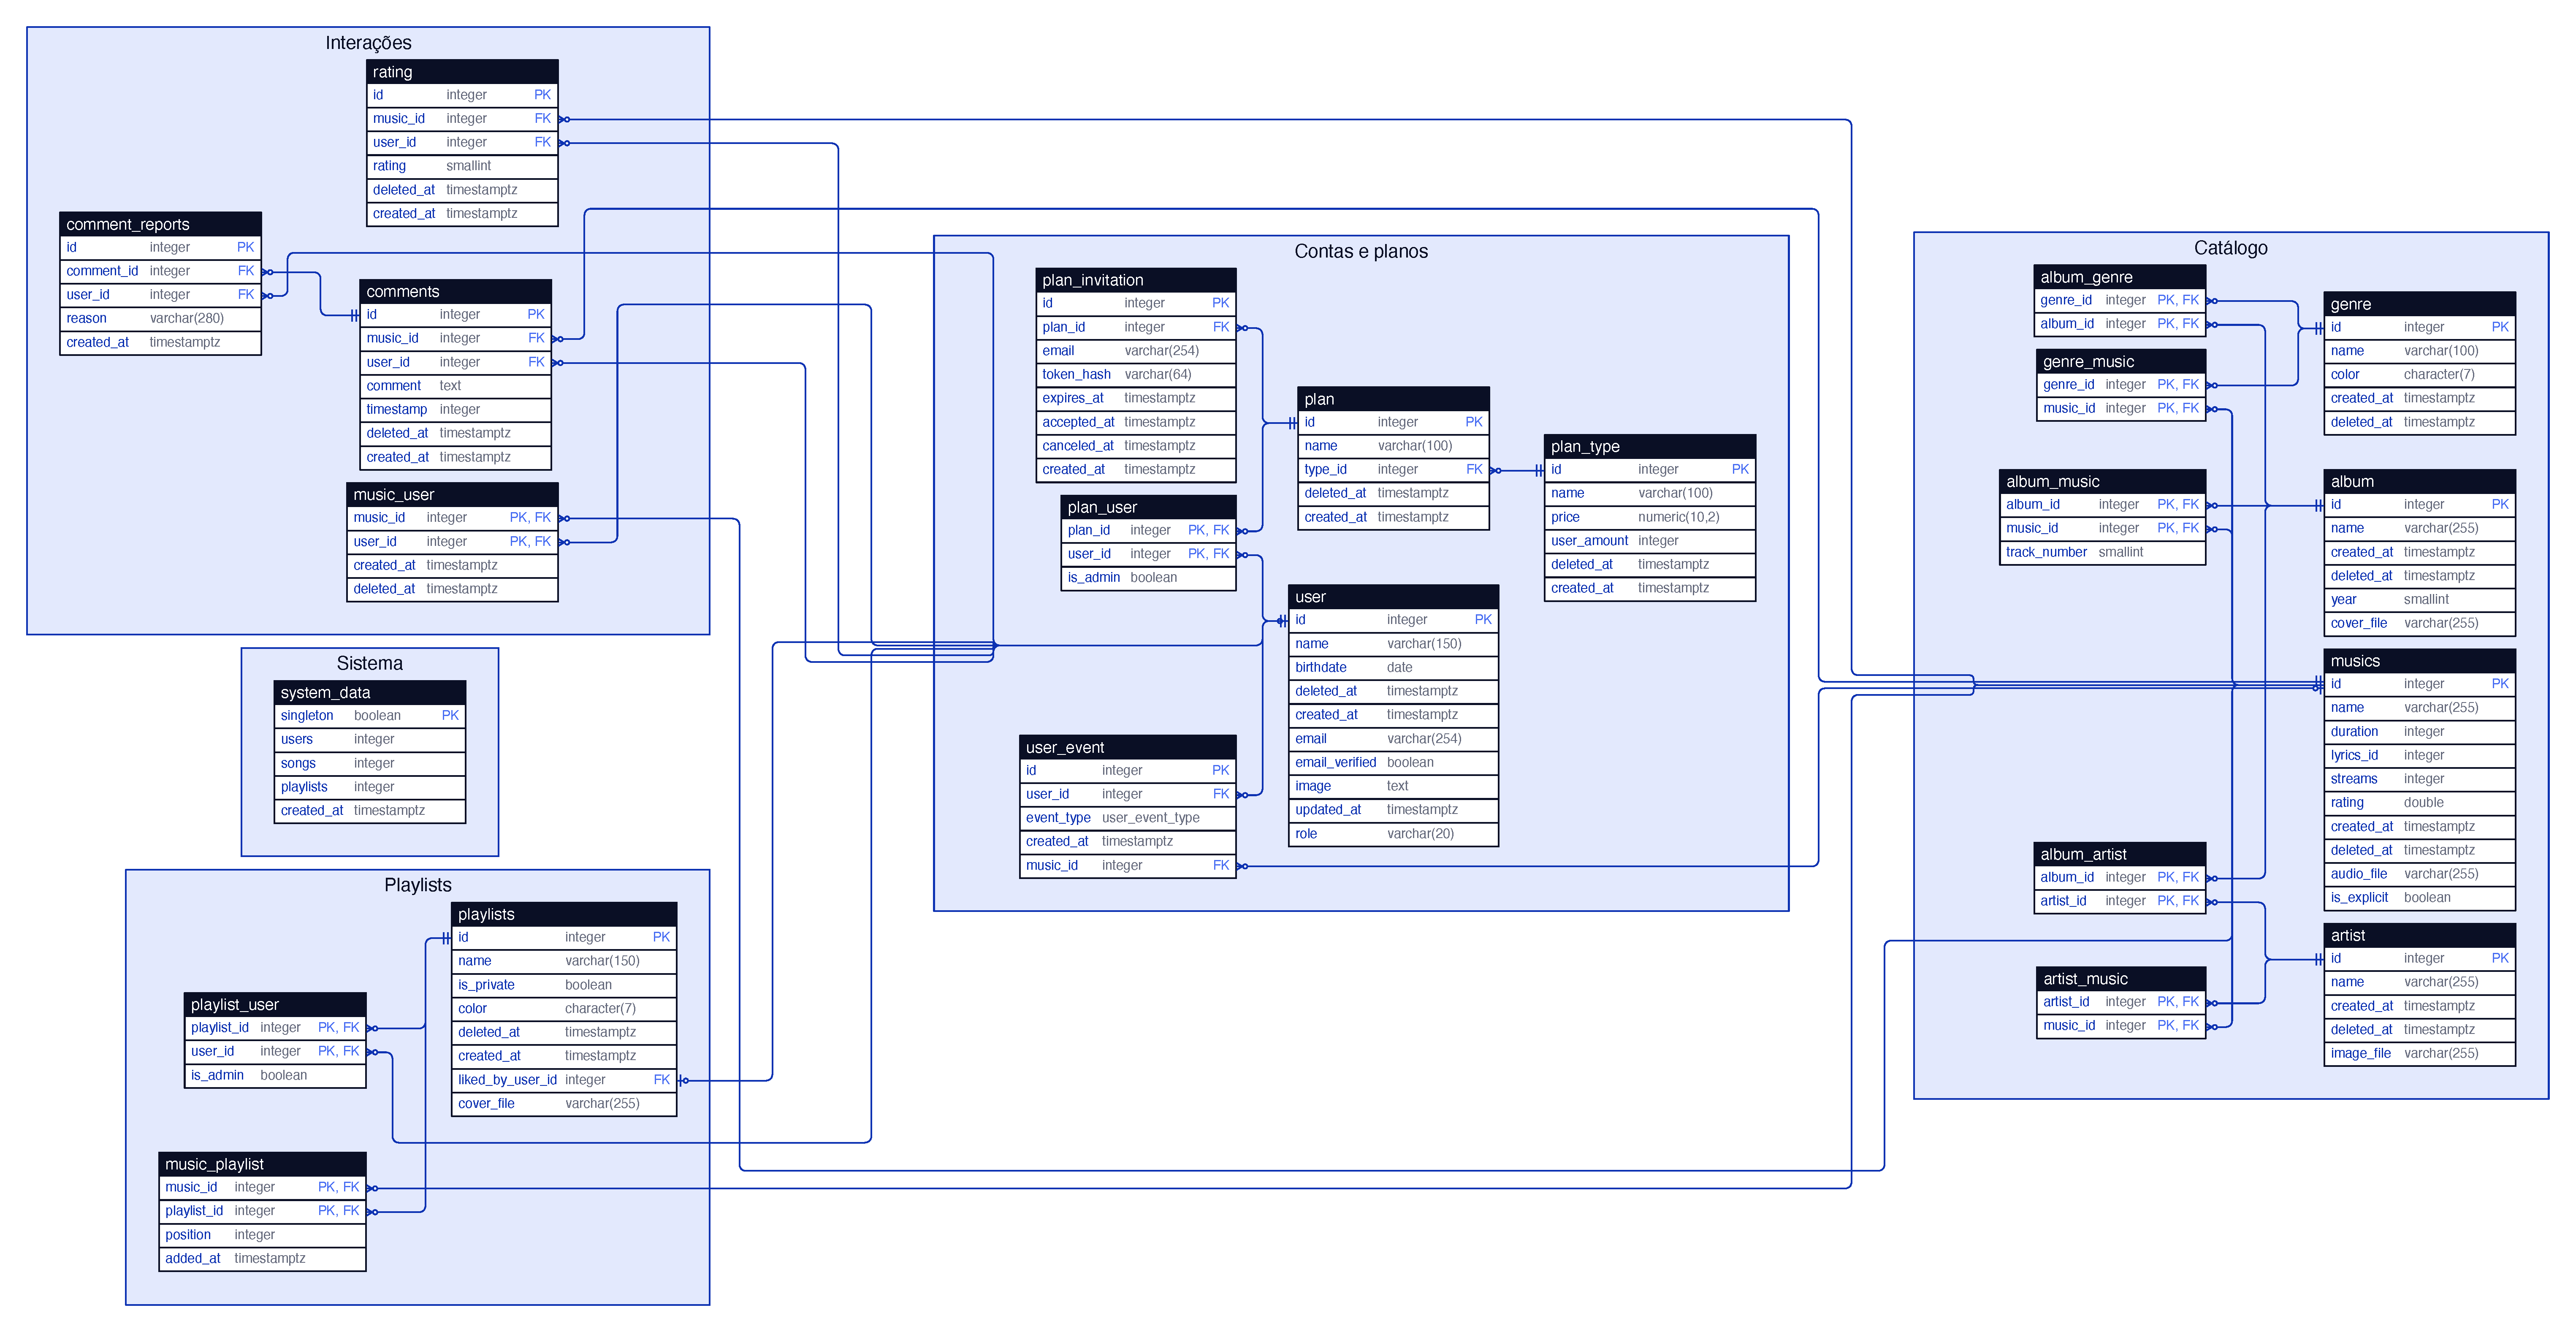
\includegraphics[width=\textwidth]{figuras/modelo-relacional.pdf}
  \caption{Modelo relacional, gerado a partir do próprio banco pelo script
    \campo{db:erd} (sem as tabelas do Better Auth)}
  \label{fig:relacional}
\end{figure}

A \cref{fig:relacional} não é desenhada à mão. O script \campo{db:erd} lê as
tabelas, colunas e chaves do catálogo do Postgres e desenha o diagrama com o
D2. O GitHub Actions o executa a cada push, então a figura sempre corresponde
ao banco.

\FloatBarrier
\subsection{Tabelas}

\begin{table}[htbp]
  \centering
  \caption{Tabelas do banco, por área}
  \label{tab:tabelas}
  \small
  \begin{tabularx}{\textwidth}{@{}L{0.6}L{0.9}L{1.5}@{}}
    \toprule
    \poliCabTabela{Área} & \poliCabTabela{Tabela} & \poliCabTabela{O que guarda} \\
    \midrule
    Contas e planos & \campo{user} & As contas; é também a tabela de usuários do Better Auth \\
     & \campo{plan\_type} & Os tipos de plano, com preço e limite de pessoas \\
     & \campo{plan} & Os planos assinados \\
     & \campo{plan\_user} & Quem está em cada plano e quem é o gestor (\campo{is\_admin}) \\
     & \campo{plan\_invitation} & Os convites do plano familiar \\
     & \campo{user\_event} & Os eventos de uso, com a música quando é uma reprodução \\
     & \campo{system\_data} & Contadores gerais do sistema, numa única linha \\
    \midrule
    Catálogo & \campo{musics} & As músicas \\
     & \campo{album}, \campo{artist}, \campo{genre} & Os álbuns, os artistas e os gêneros \\
     & \campo{album\_music} & As faixas de cada álbum, com \campo{track\_number} \\
     & \campo{artist\_music}, \campo{album\_artist} & Os artistas de cada música e de cada álbum \\
     & \campo{genre\_music}, \campo{album\_genre} & Os gêneros de cada música e de cada álbum \\
    \midrule
    Playlists & \campo{playlists} & As playlists \\
     & \campo{playlist\_user} & Os membros de cada playlist e quem a administra \\
     & \campo{music\_playlist} & As músicas de cada playlist, em ordem \\
    \midrule
    Interações & \campo{rating} & As avaliações de 1 a 5 \\
     & \campo{music\_user} & As músicas salvas por cada conta \\
     & \campo{comments} & Os comentários \\
     & \campo{comment\_reports} & As denúncias de comentários, com o motivo \\
    \midrule
    Autenticação & \campo{session} & As sessões abertas; o \campo{token} é o valor do cookie \\
     & \campo{account} & Uma linha por forma de login; com email e senha, guarda o hash \\
     & \campo{verification} & Tokens de confirmação de email e recuperação de senha \\
    \bottomrule
  \end{tabularx}
\end{table}

\FloatBarrier
\subsection{Convenções}

\begin{itemize}
  \item \textbf{Nomes} em inglês e \emph{snake\_case}. As constraints seguem o
    padrão do Prisma (\campo{<tabela>\_pkey}, \campo{<tabela>\_<coluna>\_fkey}),
    para que o \campo{schema.prisma} gerado não precise de mapeamentos.
  \item \textbf{Datas} em \campo{timestamptz}, com fuso. As tabelas registram
    \campo{created\_at} e, quando há remoção lógica, \campo{deleted\_at}. Só
    as tabelas do Better Auth têm \campo{updated\_at}, porque a biblioteca
    atualiza esses registros.
  \item \textbf{Arquivos} (áudio das músicas, capas e fotos) ficam fora do
    banco, num diretório do servidor. O banco guarda só o nome do arquivo
    (\campo{<uuid>.mp3}), para que o diretório possa mudar sem migrar dados.
  \item \textbf{Senhas e tokens} nunca são guardados em texto puro. A senha
    fica em \campo{account.password} com hash \emph{scrypt}, e o convite
    guarda só o hash SHA-256 do token do link.
\end{itemize}

\section{Restrições de Integridade}
\label{sec:integridade}

As regras de formato e de valor são garantidas pelo próprio banco, e não só
pela API. Assim, um dado inválido não entra nem por um script, nem por uma
consulta manual, nem por um bug.

\subsection{Chaves estrangeiras}

Toda chave estrangeira tem uma ação definida para quando a linha referenciada
é apagada:

\begin{itemize}
  \item \campo{ON DELETE CASCADE} nas tabelas associativas e nas que dependem
    de um dono: apagar uma playlist apaga os vínculos dela com músicas e
    membros. Na prática, isso quase nunca acontece, porque a aplicação usa
    remoção lógica.
  \item \campo{ON DELETE RESTRICT} em \campo{plan.type\_id}: um tipo de plano
    em uso não pode ser apagado.
\end{itemize}

\subsection{Restrições \texttt{CHECK}}

Cada \campo{CHECK} recusa a linha que viola a regra, com um erro que a API
traduz para a pessoa. A \cref{tab:checks} lista as principais.

\begin{table}[htbp]
  \centering
  \caption{Principais restrições \texttt{CHECK}}
  \label{tab:checks}
  \small
  \begin{tabularx}{\textwidth}{@{}L{0.9}L{1.1}@{}}
    \toprule
    \poliCabTabela{Restrição} & \poliCabTabela{Regra} \\
    \midrule
    \campo{rating BETWEEN 1 AND 5} & Nota da avaliação e média da música \\
    \campo{duration > 0} & Toda música tem duração positiva, em segundos \\
    \campo{price >= 0}, \campo{user\_amount > 0} & Preço e limite de pessoas do tipo de plano \\
    \campo{color \textasciitilde{} '\^{}\#[0-9A-Fa-f]\{6\}\$'} & Cores de gênero e de playlist no formato \campo{\#RRGGBB} \\
    \campo{email = lower(email)} & Emails de contas e de convites sempre em minúsculas \\
    \campo{role IN ('admin', 'assinante')} & Papéis possíveis de uma conta \\
    \campo{year >= 1900} & Ano do álbum; o limite ``até o ano atual'' fica no domínio, porque muda com o tempo \\
    \campo{track\_number > 0}, \campo{position >= 0} & Número da faixa no álbum e posição na playlist \\
    \campo{music\_id IS NULL OR event\_type IN (...)} & Só eventos de reprodução (\campo{music\_play}, \campo{music\_skip}, \campo{music\_listened}) apontam para uma música \\
    \campo{CHECK (singleton)} & \campo{system\_data} tem uma única linha \\
    \bottomrule
  \end{tabularx}
\end{table}

\FloatBarrier
\subsection{Unicidade}

Várias regras de unicidade valem só entre os registros ativos. Elas usam
\textbf{índices únicos parciais}, com \campo{WHERE deleted\_at IS NULL}, para
que um registro removido não bloqueie um novo:

\begin{itemize}
  \item nome de gênero único entre os ativos;
  \item nome de artista único entre os ativos, sem diferenciar maiúsculas de
    minúsculas (índice sobre \campo{lower(name)});
  \item uma avaliação ativa por pessoa e música.
\end{itemize}

Outras são \campo{UNIQUE} comuns: o email da conta (que continua reservado
mesmo depois da remoção), o token da sessão, o hash do token do convite, a
playlist de curtidas de cada conta e a denúncia de uma pessoa para um
comentário.

Duas unicidades de posição merecem destaque. O número da faixa é único dentro
do álbum (\campo{UNIQUE (album\_id, track\_number)}), e a posição é única
dentro da playlist. Na playlist, a constraint é \campo{DEFERRABLE INITIALLY
DEFERRED}: reordenar as músicas troca as posições num único \campo{UPDATE}, e
duas músicas passam um instante pela mesma posição. Com a verificação adiada,
o Postgres só confere a regra no \campo{COMMIT}.

\begin{listing}[htbp]
  \caption{Tabela de convites do plano familiar
    (\campo{V261105\_151000\_\_Adiciona\_convites\_do\_plano.sql})}
  \label{cod:convite}
  \begin{minted}{sql}
CREATE TABLE plan_invitation (
    id          integer      GENERATED BY DEFAULT AS IDENTITY,
    plan_id     integer      NOT NULL,
    email       varchar(254) NOT NULL,
    token_hash  varchar(64)  NOT NULL,
    expires_at  timestamptz  NOT NULL,
    accepted_at timestamptz,
    canceled_at timestamptz,
    created_at  timestamptz  NOT NULL DEFAULT now(),
    CONSTRAINT plan_invitation_pkey PRIMARY KEY (id),
    CONSTRAINT plan_invitation_token_hash_key UNIQUE (token_hash),
    CONSTRAINT plan_invitation_email_lower_check CHECK (email = lower(email)),
    CONSTRAINT plan_invitation_plan_id_fkey FOREIGN KEY (plan_id)
        REFERENCES plan (id) ON DELETE CASCADE
);
  \end{minted}
\end{listing}

O \cref{cod:convite} reúne os elementos desta seção: chave primária gerada,
chave estrangeira com ação definida, \campo{UNIQUE} e \campo{CHECK}, todos com
nome no padrão do projeto. O estado do convite não é uma coluna: ele está
pendente enquanto \campo{accepted\_at} e \campo{canceled\_at} são nulos e
\campo{expires\_at} está no futuro.

\FloatBarrier
\subsection{Regras que ficam no domínio}

Algumas regras dependem de contar linhas ou do momento atual, e um
\campo{CHECK} não as expressa. Elas são verificadas nos casos de uso da API:

\begin{itemize}
  \item todo plano tem ao menos uma pessoa, e o Família não passa de quatro,
    contando os convites pendentes;
  \item toda música e todo álbum têm ao menos um artista;
  \item toda playlist tem ao menos um membro;
  \item o ano do álbum não passa do ano atual;
  \item uma música só conta como ouvida com mais de 30 segundos de reprodução
    (\campo{LISTENED\_THRESHOLD\_SECONDS}).
\end{itemize}

\section{Evolução do Esquema}
\label{sec:evolucao}

O esquema muda ao longo do projeto: cada funcionalidade nova pode pedir uma
tabela ou uma coluna. Essas mudanças são feitas por \textbf{migrations} do
Flyway, arquivos SQL aplicados em ordem e registrados na tabela
\campo{flyway\_schema\_history}. O Flyway roda a cada \campo{docker compose
up}, então o banco de qualquer integrante e o de produção ficam sempre na
mesma versão.

\subsection{Nome e ordem}

O nome de cada arquivo segue o padrão
\campo{V<AAMMDD>\_<HHMMSS>\_\_<Descricao>.sql}. Como a versão é a data e a hora
de criação, as migrations de integrantes diferentes não disputam o mesmo
número, e rodam na ordem em que foram escritas. Um nome fora do padrão faz o
Flyway falhar (\campo{validateMigrationNaming}), em vez de ignorar o arquivo em
silêncio.

\begin{table}[htbp]
  \centering
  \caption{Migrations aplicadas até a entrega}
  \label{tab:migrations}
  \small
  \begin{tabularx}{\textwidth}{@{}L{0.42}L{1.58}@{}}
    \toprule
    \poliCabTabela{Versão} & \poliCabTabela{O que muda} \\
    \midrule
    \campo{V1} & Esquema inicial: planos, usuários, catálogo, interações e playlists \\
    \campo{V261020\_162546} & Tabelas do Better Auth e email na tabela \campo{user} \\
    \campo{V261026\_133836} & Papel do usuário (\campo{admin} ou \campo{assinante}) \\
    \campo{V261103\_151718} & Extensão \campo{unaccent}, para a busca não diferenciar acentos \\
    \campo{V261103\_154132} & Eventos de reprodução passam a apontar para a música \\
    \campo{V261103\_163300} & Ordem das músicas na playlist \\
    \campo{V261105\_151000} & Convites do plano familiar e limite de 4 pessoas \\
    \campo{V261105\_162500} & Denúncias de comentários \\
    \campo{V261105\_183723} & Áudio e conteúdo explícito na música, ano no álbum \\
    \campo{V261105\_213000} & Capa do álbum \\
    \campo{V261112\_120000} & Número da faixa no álbum \\
    \campo{V261115\_200000} & Playlist ``Músicas Curtidas'' de cada conta \\
    \campo{V261116\_090000} & Evento \campo{music\_listened} \\
    \campo{V261116\_090100} & O evento \campo{music\_listened} também leva a música \\
    \campo{V261117\_160000} & Nome de artista único, com a fusão dos duplicados \\
    \campo{V261117\_170000} & Capa da playlist e foto do artista \\
    \bottomrule
  \end{tabularx}
\end{table}

\FloatBarrier
\subsection{Regras}

\begin{itemize}
  \item \textbf{Uma migration publicada nunca é editada.} O Flyway guarda um
    checksum de cada arquivo aplicado e se recusa a subir se ele mudar. Uma
    correção é sempre uma migration nova.
  \item \textbf{Dados de teste não entram em migration}, porque as migrations
    também rodam em produção. Eles ficam no seed (\cref{sec:acesso}).
  \item \textbf{Uma regra nova cuida dos dados que já existem.} Antes de criar
    o índice de nome de artista único, a migration
    \campo{V261117\_160000} funde os artistas de mesmo nome no de menor
    \campo{id}: os vínculos com álbuns e músicas passam para ele, e os outros
    recebem remoção lógica. Sem isso, o índice falharia em bancos que já
    tivessem duplicados.
  \item \textbf{Valor novo de enum e o uso dele vão em migrations separadas.}
    O Postgres não permite usar um valor de enum na mesma transação em que ele
    foi criado, e o Flyway roda cada migration numa transação. Por isso
    \campo{music\_listened} entrou numa migration, e o \campo{CHECK} que o usa
    entrou na seguinte.
\end{itemize}

\subsection{Documentação gerada}

Depois de uma migration, o comando \campo{db:sync} atualiza o
\campo{schema.prisma} a partir do banco, e o \campo{db:sync --check} confere se
os dois estão iguais. O diagrama da \cref{fig:relacional} é gerado pelo CI.
Com isso, a documentação do esquema não depende de alguém lembrar de
atualizá-la.

\section{Acesso aos Dados}
\label{sec:acesso}

\subsection{Pela API}

A API abre um \emph{pool} de até dez conexões com o driver \campo{pg}, com
tempo limite de 5 segundos para conectar e de 10 segundos por
consulta. Cada repositório em \campo{api/adapters/db} escreve o próprio SQL,
com parâmetros (\campo{\$1}, \campo{\$2}) em vez de concatenação de texto, o
que impede injeção de SQL.

Operações com mais de um passo rodam numa transação, pela função
\campo{inTransaction}: ou tudo é gravado, ou nada. É o caso de salvar uma música,
que grava a linha em \campo{musics} e regrava os artistas, os gêneros e a faixa
no álbum, e de criar um convite do plano familiar.

O convite mostra por que só a transação não basta. O limite de quatro pessoas
conta os membros e os convites pendentes, e duas requisições simultâneas
poderiam contar a mesma vaga livre e criar um convite cada uma. Para evitar
isso, a transação começa com um \emph{lock} consultivo do Postgres
(\campo{pg\_advisory\_xact\_lock}) com o \campo{id} do plano: o segundo
convite espera o primeiro terminar e já enxerga a vaga ocupada.

As colunas \campo{date}, como a data de nascimento, voltam como texto
(\campo{AAAA-MM-DD}). O conversor padrão do driver as transformaria em
meia-noite no fuso do servidor, e a data poderia mudar de dia. Isso afetaria
a regra de idade do conteúdo explícito.

\subsection{Seed}

O seed, em \campo{api/prisma/seed/}, popula o banco com o client do Prisma.
Cada seeder tem um ambiente:

\begin{itemize}
  \item \textbf{ALL}: dados reais do produto, como os tipos de plano e os
    gêneros. Rodam no banco local e em produção, e nunca apagam nada.
  \item \textbf{LOCAL}: dados fictícios para desenvolver e testar (usuários,
    catálogo, playlists e interações). Só rodam num banco em
    \campo{localhost}.
\end{itemize}

O seed roda numa transação e usa uma semente fixa, então gera os mesmos dados
e os mesmos \campo{id}s em todas as máquinas. Isso torna os testes manuais
reproduzíveis entre os integrantes.

\subsection{Ambientes}

Localmente, o Postgres roda num contêiner Docker, acessível só pela própria
máquina. Em produção, o banco roda no servidor da equipe e não é exposto à
internet: o acesso passa por um túnel da Cloudflare protegido pelo Cloudflare
Access, liberado só para os emails da equipe. Os usuários do Postgres da
equipe podem ler e alterar dados, mas não mudar o esquema, que é papel das
migrations, nem ler as tabelas com tokens e hashes de senha.

\section{Limitações e Próximos Passos}
\label{sec:limitacoes}

A revisão do modelo conceitual mostrou pontos em que o banco atual guarda
mais do que o modelo pede. Eles estão listados abaixo, com a mudança
planejada.

\begin{table}[htbp]
  \centering
  \caption{Pontos em aberto no esquema}
  \label{tab:pendencias}
  \small
  \begin{tabularx}{\textwidth}{@{}L{0.8}L{1.15}L{1.05}@{}}
    \toprule
    \poliCabTabela{Ponto} & \poliCabTabela{Problema} & \poliCabTabela{Mudança planejada} \\
    \midrule
    \campo{musics.rating} e \campo{musics.streams} & Dados derivados: repetem a média de \campo{rating} e a contagem de \campo{user\_event}, e podem divergir delas & Calcular na consulta e apagar as colunas \\
    \campo{rating} (nota de 1 a 5) & A HU-20 trocou a nota por like e dislike & Tabela de votos no lugar de \campo{rating} \\
    \campo{system\_data} & Contadores que um \campo{COUNT} já calcula; hoje só o seed escreve nela & Apagar a tabela ou trocá-la por uma \emph{view} \\
    \campo{music\_user} & As curtidas passaram para a playlist ``Músicas Curtidas'', e a API não usa mais a tabela & Apagar a tabela \\
    \campo{musics.lyrics\_id} & Coluna sem chave estrangeira: a tabela de letras ainda não existe & Criar a tabela de letras, se a funcionalidade entrar no escopo \\
    \bottomrule
  \end{tabularx}
\end{table}

Cada mudança será uma migration nova, seguindo as regras da
\cref{sec:evolucao}. Quando uma delas for aplicada, o modelo relacional da
\cref{fig:relacional} se atualiza sozinho no próximo push, e o modelo
conceitual da \cref{fig:der} já está na forma final.


\end{document}
